%****************************************************
%	CHAPTER 3 - Dynamics
%****************************************************
\chapter{Kinematics \& Dynamics}
\label{ch:dynamics}
%====================================================
Generally applicable rigid body dynamics are first derived. Thereafter, those dynamics are adapted to the non-linear multibody case where constrained relative internal rotational in permitted. Following that, aerodynamic effects are investigated and incorporated into the plant's model. Finally a consolidated, quaternion based plant model is presented which is used for the later control plant development next in Chapter:\ref{ch:control}.
%====================================================
\section{Rigid Body Dynamics}
\label{sec:dynamics.rigidbody}
%====================================================
\subsection{Lagrange Derivation}
\label{subsec:dynamics.rigidbody.lagrange}
%====================================================
Fundamentally any body, rigid or otherwise, can undergo two kinds of movements, namely rotational and translation motions. Often a Lagrangian\cite{classicaldynamics,rotationrigidbody} approach for combined angular and translational movements is used to derive the differential equations of motion for each degree of freedom. The Lagrangian principle ensures that (translational and rotational) kinematic energies and potential energy are conserved throughout the system's trajectory progression. When combined with Euler-Rotational equations, the Euler-Lagrangian\cite{lagrange-formalism} formulation fully defines the aerospace 6-DOF equation set.
\par
Lagrangian formalism is regarded as especially useful in non-cartesian (\emph{spherical etc\ldots}) co-ordinate frames or multi-body systems. With that being said, a cartesian co-ordinate system was already defined in Section:\ref{subsec:proto.conventions.motoraxis}. Rigid body dynamics in a cartesian co-ordinate frame do lend themselves to Newtonian mechanics. The Newton-Euler or Euler-Lagrange formulations both stipulate the same resultant differential equations of motion. The Lagrangian operator, $\mathcal{L}$, is a term consisting of the difference between kinetic and potential energies, $T$ and $U$ respectively. Considering some generalized path co-ordinates $\mathbf{r}(t)$, for both linear $\vec{\mathcal{E}}$ and angular $\vec{\eta}$ relative positions;
\begin{equation}\label{eq:generalpath}
\mathbf{r}(t)=\begin{bmatrix}
\vec{\mathcal{E}} \\
\vec{\eta}
\end{bmatrix}
\end{equation}
The co-ordinates in Eq:\ref{eq:generalpath} are generalized here, despite being symbols commonly used to represent linear and angular positions. The generalized co-ordinates are later be refined as Cartesian body co-ordinates with respect to the inertial frame. The Lagrangian is, by definition:
\begin{subequations}
\begin{equation}\label{eq:lagrangian.a}
\mathcal{L}(\mathbf{r},\dot{\mathbf{r}},t)=T(\mathbf{r},\dot{\mathbf{r}})-U(\mathbf{r},\dot{\mathbf{r}})
\end{equation}
With kinetic and potential energy function(s) $T$ and $U$ respectively. Then introducing a rigid body's general kinetic (angular \& linear) and potential energies, in some shared reference frame. In this case the only potential energy is gravitational\footnote{Here $G=\begin{bmatrix}
0&0&-9.81
\end{bmatrix}^T~m.s^{-2}$~in the Inertial frame,$\in\mathcal{F}^I$} potential energy:
\begin{equation}\label{eq:lagrangian.b}
\mathcal{L}=
\frac{1}{2}
\begin{bmatrix}
\dot{\vec{\mathcal{E}}}^{~T}(m)\dot{\vec{\mathcal{E}}}\\
\dot{\vec{\eta}}^{~T}(\mathbb{I}_b)\dot{\vec{\eta}}
\end{bmatrix}
-
\begin{bmatrix}
m\vec{G}z\\
0
\end{bmatrix}
\end{equation}
\end{subequations}
Noting that $\mathbb{I}_b$ is the inertial tensor of the body aligned w.r.t to whichever reference frame is used. The Euler-Lagrange formulation equates partial derivatives of the Lagrangian to any generalized forces, $\mathbf{V}$, acting on the system. In this case the generalized forces or, more specifically a net force $\vec{F}_{net}$ and a net torque $\vec{\tau}_{net}$.
\begin{equation}\label{eq:euler-lagrange}
\frac{d}{dt}\bigg(\frac{\delta L}{\delta \dot{\mathbf{r}}}\bigg)-\frac{\delta L}{\delta \mathbf{r}} = \mathbf{V} = \begin{bmatrix}
\vec{F}_{net}\\
\vec{\tau}_{net}
\end{bmatrix}
\end{equation}
And taking the partial derivatives of Eq:\ref{eq:lagrangian.b} with respect to the path co-ordinates $\mathbf{r}$:
\begin{subequations}
\begin{equation}\label{eq:partial.a}
\frac{\delta L}{\delta \mathbf{r}}=\begin{bmatrix}
m\vec{G}_x\\
0
\end{bmatrix}
\end{equation}
\vspace{-5pt}
\begin{equation}\label{eq:partial.b}
\frac{d}{dt}\bigg(\frac{\delta L}{\delta \dot{\mathbf{r}}}\bigg)=\bigg[
m\frac{d}{dt}\dot{\vec{\mathcal{E}}} ~~~ \mathbb{I}\frac{d}{dt}\dot{\vec{\eta}}\bigg]^T
\end{equation}
\end{subequations}
Where $\vec{G}_x$ is the gravitation force in whichever reference frame ($\mathcal{F}^x$) the lagrangian is with respect to. In any generalized coordinate system a rotating vector's time derivative which, according to the Reynolds Transportation Theorem\cite{reynolds}, is given by:
\begin{equation}\label{eq:reynolds}
\frac{d\vec{f}}{dt_a}=\frac{d\vec{f}}{dt_b}+\vec{\omega}_{a/b}\times\vec{f}
\end{equation}
So applying that theorem (Eq:\ref{eq:reynolds}) to the partial derivatives in Eq:\ref{eq:partial.b} and further defining the generalized co-ordinates as cartesian body coordinates with respect to an inertial origin (the body frame $\mathcal{F}^b$ and inertial frame $\mathcal{F}^I$). Noting that in Eq:\ref{eq:partial.b} the place holders used for linear ($\vec{\mathcal{E}}$) and angular positions ($\vec{\eta}$) all exist in a common shared frame\footnote{In this case $\vec{\eta}\not=[\phi~\theta~\psi]^T$ seeing that the angular position $\vec{\eta}$ is defined in a common frame. $\vec{\eta}$ is \underline{NOT an Euler angle} set.}, and hence:
\begin{equation}
\frac{d}{dt}
\begin{bmatrix}
{\mathcal{E}}\\
\vec{\eta}
\end{bmatrix}
\triangleq
\begin{bmatrix}
\vec{\nu}\\
\vec{\omega}
\end{bmatrix}
\in \mathcal{F}^b
\end{equation}
It then follows that the Lagrangian Eq:\ref{eq:lagrangian.b} changes to:
\begin{subequations}
\begin{equation}
\mathcal{L}=\frac{1}{2}
\begin{bmatrix}
\vec{\nu}^{~T}(m)\vec{\nu}\\
\vec{\omega}^{~T}(\mathbb{I})\vec{\omega}
\end{bmatrix}
-
\begin{bmatrix}
m\vec{G}_b z\\
0
\end{bmatrix}
\end{equation}
\vspace{-5pt}
\begin{equation}
\frac{d}{dt}\bigg(\frac{\delta L}{\delta \dot{\mathbf{r}}}\bigg)=\bigg[
m\frac{d}{dt}\vec{\nu} ~~~ \mathbb{I}\frac{d}{dt}\vec{\omega}\bigg]^T
\end{equation}
\vspace{-5pt}
\begin{equation}
\rightarrow m\frac{d}{dt}\vec{\nu}=m\dot{\vec{\nu}}+\vec{\omega}_{I/b}\times\vec{\nu}
\end{equation}
\vspace{-5pt}
\begin{equation}
\rightarrow \mathbb{I}_b \frac{d}{dt}\vec{\omega}=\mathbb{I}_b\dot{\vec{\omega}}+\vec{\omega}_{I/b}\times\mathbb{I}_b\vec{\omega}
\end{equation}
\end{subequations}
Which, when substituted back into the Euler-Lagrange formulation Eq:\ref{eq:euler-lagrange}, results in the familiar Newton-Euler equations for linear and angular differentials, both in the body frame;
\begin{subequations}\label{eq:newton}
\begin{equation}\label{eq:newton.a}
\vec{F}_{net}=m\dot{\vec{\nu}}+\vec{\omega}_b\times m \vec{\nu} - m\mathbb{R}_I^b(-\eta) \vec{G}_I
\end{equation}
\vspace{-15pt}
\begin{equation}\label{eq:newton.b}
\vec{\tau}_{net}=\mathbb{I}_b\dot{\vec{\omega}}_b+\vec{\omega}_b\times\mathbb{I}_b\vec{\omega}_b
\end{equation}
\end{subequations}
It's important to recall that $\vec{\omega}_b\not= \dot{\vec{\eta}}$ where $\vec{\eta}=[\phi~\theta~\psi]^T$, seeing that Euler Angles are defined in sequentially rotated reference frames. So then four differential equations are often used to completely describe the entire set of state derivatives, namely:
\begin{subequations}\label{eq:states}
\begin{equation}\label{eq:states.a}
\dot{\vec{\mathcal{E}}}=\mathbb{R}_b^I(-\eta)\vec{\nu}~~~~\in\mathcal{F}^I
\end{equation}
\vspace{-10pt}
\begin{equation}\label{eq:states.b}
\vec{F}_{net}=m\dot{\vec{\nu}}+\vec{\omega}_b\times m\vec{\nu} -m \mathbb{R}_I^b(-\eta)\vec{G}_I ~~~~\in\mathcal{F}^b
\end{equation}
\newpage
\begin{equation}\label{eq:states.c}
\dot{\vec{\eta}}=\Psi(\eta)\vec{\omega}_b~~~~\in\mathcal{F}^{v2},\mathcal{F}^{v1},\mathcal{F}^I
\end{equation}
\vspace{-10pt}
\begin{equation}\label{eq:states.d}
\vec{\tau}_{net}=\mathbb{I}_b\dot{\vec{\omega}}_b+\vec{\omega}_b\times\mathbb{I}_b\vec{\omega}_b~~~~\in\mathcal{F}^b
\end{equation}
\end{subequations}
The state differentials in Eq:\ref{eq:states} can be reduced to a set of two equations. Those differentials are defined in reference frames of the state variables which they represent. The non-linear form of those equations substitutes\footnote{Originally introduced in Eq:\ref{eq:angular-rates.e}} $d\vec{\eta}/dt=\Phi(\eta)\vec{\omega}_b$ in the Lagrangian derivative, Eq:\ref{eq:partial.b}.
\begin{equation}
\frac{d}{dt}\bigg(\frac{\delta \mathcal{L}}{\delta \dot{\mathbf{r}}}\bigg)=\bigg[m\frac{d}{dt}\vec{\nu}~~~\mathbb{I}\frac{d}{dt}\dot{\vec{\eta}}\bigg]^T\Rightarrow\bigg[m\frac{d}{dt}\vec{\nu}~~~\mathbb{I}\frac{d}{dt}\Phi(\eta)\vec{\omega}_b\bigg]^T
\end{equation}
This only affects the angular component as the two kinetic energies are independent of one another. And so applying the differential chain rule:
\begin{equation}
\mathbb{I}\frac{d}{dt}\Phi(\eta)\vec{\omega}_b=\mathbb{I}\big(\Phi\dot{(\eta)}\vec{\omega}_b+\Phi(\eta)\dot{\vec{\omega}}_b \big)
\end{equation}
Drawing from \cite{autonomousrobotseuler} and recognizing that $\mathbb{I}$ must be transformed to the common intermediate Euler axes, $\mathbb{J}=\Psi(\eta)^T\mathbb{I}\Psi(\eta)$. The controllable differential equation for angular acceleration in Eq:\ref{eq:newton.b}, then in intermediate Euler frames for each angle becomes\footnote{The relationship $\dot{\Phi}=\Phi\dot{\Psi}\Phi$ was used to simplify Eq:\ref{eq:nonlinear}, the singularity in $\Phi$ still remains\ldots}:
\begin{subequations}\label{eq:nonlinear}
\begin{equation}\label{eq:nonlinear.a}
M(\eta)\ddot{\vec{\eta}}+C(\eta,\dot{\eta})\dot{\vec{\eta}}=\Psi(\eta)\vec{\tau}_{net}
\end{equation}
\vspace{-15pt}
\begin{equation}\label{eq:nonlinear.b}
M(\eta)=\Psi(\eta)^T\mathbb{I}\Psi(\eta)
\end{equation}
\vspace{-10pt}
\begin{equation}\label{eq:nonlinear.c}
C(\eta,\dot{\eta})=-\Psi(\eta)\mathbb{I}\Psi\dot{(\eta)}+\Psi(\eta)^T \big[\Psi(\eta)\dot{\vec{\eta}}\big]_{\times}\mathbb{I}\Psi(\eta)
\end{equation}
\end{subequations}
Equation \ref{eq:nonlinear.a} fully describes the state derivative $\ddot{\vec{\eta}}$ in its own frame(s). The two differential equations which describe the entire bodies motion are then:
\begin{subequations}\label{eq:rigid-frame}
\begin{equation}\label{eq:rigid-frame.a}
\vec{F}_{net}=m\dot{\vec{\mathcal{E}}}+\mathbb{R}_b^I(-\eta)\vec{\omega}_b \times m \dot{\vec{\mathcal{E}}}-m\vec{G}_I~~~~\in\mathcal{F}^I
\end{equation}
\vspace{-10pt}
\begin{equation}\label{eq:rigid-frame.b}
\vec{\tau}_{net}=\Psi(\eta)^{-1}M(\eta)\ddot{\vec{\eta}}+\Psi(\eta)^{-1}C(\eta,\dot{\eta})~~~~\in\mathcal{F}^{v2,v1,I}
\end{equation}
\end{subequations}
\par
The generalized net forces effecting the system, $\vec{F}(u)$ and $\vec{\tau} (u)$, are the system's controllable inputs and are going to be affected directly the systems actuators and their associated effectiveness function. In the general case, which is expanded upon in Section:\ref{sec:dynamics.aero}, the control inputs are typically as follows:
\begin{subequations}
The net force acting on the system is just the sum of all thrust vectors produced by rotating propellers, $T(\Omega_i)$.
\begin{equation}
\mu \vec{F} = \sum_{i=1}^4 \vec{T}(\Omega_i)
\end{equation}
Secondly the net torque is the sum of all torque arms produced from those propeller thrust vectors.
\begin{equation}
\mu \vec{\tau} = \sum_{i=1}^4 \vec{l}_i \times \vec{T}(\Omega_i)
\end{equation}
\end{subequations}
Where $\vec{T}(\Omega_i)$ is the $i^{th}$ motor's thrust vector, not necessarily in $\mathbb{R}^3$, and typically bound to the $\hat{Z}_b$ axis, $\vec{l}_i$ is that thrust vector's perpendicular displacement from the origin $\mathbf{O}_b$. The above equations are still applicable to any 6 DOF body, common simplifications applied to the system(s) for quadrotor control are explored in Appendix:\ref{app:stddynamics}. Aspects unique to (multibody) aerospace frames are now introduced. Obviously the focus is on quadrotor and tilting quadrotor platforms\ldots
%====================================================
\subsection{Rotation Matrix Singularity}\label{subsec:dynamics.rigidbody.singularity}
%====================================================
The Euler Angle singularity is often mentioned but far less common is the demonstration of exactly how that singularity \emph{mathematically} manifests itself. By definition, a singularity occurs when a loss of differentiability is encountered. In the case of an affixed 3-axis gimbal (Fig:\ref{fig:gimbal}), when an intermediary rotational angle, for example the rolling angle $\theta$, is at $\pi/2$ then the remaining two axes become co-linear (Fig:\ref{fig:gimbal-lock}). That being both pitch $\phi$ or yaw $\psi$ rotations will subsequently have the same effect. Such a situation results in what is termed as a loss of a degree of freedom.
\begin{figure}[htbp]
\begin{subfigure}{0.5\textwidth}
\centering
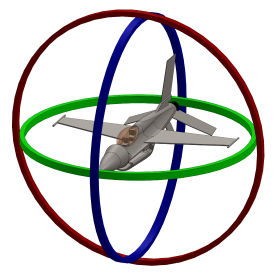
\includegraphics[width=\textwidth]{figs/gimbal}
\caption{3-Axis gimbal}
\label{fig:gimbal}
\end{subfigure}
\begin{subfigure}{0.5\textwidth}
\centering
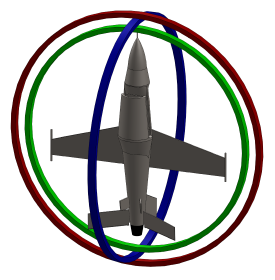
\includegraphics[width=\textwidth]{figs/gimbal-lock}
\caption{Locked gimbal with loss of DOF}
\label{fig:gimbal-lock}
\end{subfigure}
\caption{Gimbal lock}
\end{figure} 
\par
What is clear in a physical system is not necessarily as clear mathematically. An obvious loss of differentiability is manifested in the Euler Matrix $\Psi(\eta)$, Eq:\ref{eq:angular-rates.e} from Section:\ref{subsec:proto.conventions.frames}. The relation between angular velocity, in the inertial frame or inversely in the body frame, and the angular rates of the Euler Angles.
\begin{equation}\label{eq:euler-derivative}
\begin{bmatrix}
\dot{\phi}\\
\dot{\theta}\\
\dot{\psi}
\end{bmatrix}
=\begin{bmatrix}
1 & sin(\phi)tan(\theta) & cos(\phi)tan(\theta)\\
0 & cos(\phi) & -sin(\phi)\\
0 & sin(\phi)sec(\theta) & cos(\phi)sec(\theta)\\
\end{bmatrix}
\begin{bmatrix}
p\\
q\\
r
\end{bmatrix}
=\Phi(\eta)\omega_b
\end{equation}
\begin{equation}
\text{As}~\underset{{\theta \rightarrow \pi /2}}{lim}~sec(\theta),tan(\theta)\rightarrow \infty
\end{equation}
Or that $\Phi(\eta)$ is undefined at $\theta=\pi/2$. 
It's clear to see that in Eq:\ref{eq:euler-derivative} there exists an undefined singularity as $\theta\rightarrow\pi/2$. The physical consequence of this is the loss of a degree of freedom. More specifically, if one looks at how the Z-Y-X rotation (or transformation) matrices are formulated:
\begin{subequations}
\begin{equation}
\mathbb{R}_I^b = \mathbb{R}_z\mathbb{R}_y\mathbb{R}_x=\begin{bmatrix}
c_\psi & -s_\psi & 0\\
s_\psi & c_\psi & 0\\
0 & 0 & 1
\end{bmatrix}
\begin{bmatrix}
c_\theta & 0 & s_\theta\\
0 & 1 & 0\\
-s_\theta & 0 & c_\theta
\end{bmatrix}
\begin{bmatrix}
1 & 0 & 0\\
0 & c_\phi & -s_\phi\\
0 & s_\phi & c_\phi
\end{bmatrix}
\end{equation}
\begin{equation}
\mathbb{R}_I^b=\begin{bmatrix}
c_\psi c_\theta & c_\psi s_\theta s_\phi - s_\psi c_\phi & c_\psi s_\theta c_\phi + s_\psi s_\phi\\
s_\psi c_\theta & s_\psi s_\theta s_\phi + c_\psi c_\phi & s_\psi s_\theta  c_\phi - c_\psi s_\phi\\
-s_\theta & c_\theta s_\phi & c_\phi c_\theta\\
\end{bmatrix}
\end{equation}
In the case where $\theta=\pi/2$, and using trigonometric double angles;
\begin{equation}\label{eq:gimbal}
=\begin{bmatrix}
0 & c_\psi s_\phi - s_\psi c_\phi & c_\psi c_\phi + s_\psi s_\phi\\
0 & s_\psi s_\phi + c_\psi c_\phi & s_\psi c_\phi - c_\psi s_\phi\\
-1 & 0 & 0\\
\end{bmatrix}
=
\begin{bmatrix}
0 & s(\phi - \psi) & c(\phi - \psi)\\
0 & c(\phi - \psi) & s(\phi - \psi)\\
-1 & 0 & 0
\end{bmatrix}=\mathbb{R}_{x'}(\phi-\psi)
\end{equation}
\end{subequations}
Where the resultant in Eq:\ref{eq:gimbal} represents an X-axis rotation in a new intermediate frame, post a $\pi/2$ rotation in the y-axis. Through trigonometric double angles a degree of freedom is lost at $\theta=\pi/2$, when $\phi$ \& $\psi$ effect the same angle.
%====================================================
\subsection{Quaternion Dynamics}
\label{subsec:dynamics.rigidbody.quaternion}
%====================================================
An algorithm proposed in \emph{How To Avoid a Singularity When Using Euler Angles?}\cite{euleranglesingularity} suggested a solution to the problem of Euler Angle singularities. The proposed heuristic was to switch between sequencing conventions (ZYX,ZYZ etc\ldots there are 12 in total) such that the singularity is always avoided. However the implementation of such an algorithm is cumbersome and inefficient. Far more elegant is the use of \emph{quaternion} attitude representations in $\mathbb{R}^4$ (\cite{rotationsequences,quaterniondynamics,spacecraftattitutdequaternions} amongst others\ldots).
\par
A quaternion is analogous to a rotation matrix in that it represents an attitude difference between two reference frames. An $\mathbb{R}^3$ position is paramterized as a single rotation $\theta$ about a unit axis $\hat{u}$ (Sic Rodriguez Formula\cite{unwinding}). Without deliberating too much on their proof or details, a quaternion consists or a scalar component, $q_0$, and complex vector component, $\vec{q}\in \mathbb{C}^3$, such that;
\begin{equation}
Q\triangleq 
\begin{bmatrix}
q_0 \\
\vec{q}
\end{bmatrix}
~~\in\mathbb{R}^4
\end{equation}
The relationship between an Euler Angles rotation matrix $\mathbb{R}_I^b(\eta)$ and a quaternion attitude $Q_b$ is given by the Rodriguez formula:
\begin{equation}\label{eq:rodriguez}
\mathbb{R}_I^b(\eta)=\mathbb{R}(Q_b)=\mathbb{I}+2q_0[\vec{q}~]_\times+2[\vec{q}~]^2_\times
\end{equation}
Any and all quaternions, unless otherwise stated, in this dissertation are all unit quaternions\footnote{Unit quaternions are a subset of the quaternion space}, $Q\in\mathbb{Q}_u$. The need for quaternions with unity magnitude is such to ensure rotational operations don't affect the magnitude of the vector operand. A unit quaternion is defined as:
\begin{equation}
||Q||=\sqrt{{q_0}^2+\vec{q}~^2}=1
\end{equation}
Quaternion multiplication is distributive and associative, but not commutative. Specifically a quaternion multiplciation operation is equivalent to the Hamilton product. For two quaternions, $Q$ \& $P$:
\begin{subequations}
\begin{equation}
Q\otimes P = \begin{bmatrix}
q_0 \\
\vec{q}
\end{bmatrix}
\otimes
\begin{bmatrix}
p_0 \\
\vec{p}
\end{bmatrix}
\end{equation}
\vspace{-5pt}
\begin{equation}
=q_0 p_0 - \vec{q}\cdot \vec{p}+p_0 \vec{q} + q_0 \vec{p} + \vec{q}\times\vec{p}
\end{equation}
\end{subequations}
Seeing that the vector component of a quaternion is complex valued, it is natural that there exists a quaternion conjugate property. Namely:
\begin{equation}
Q^*=\begin{bmatrix}
q_0 \\
-\vec{q}
\end{bmatrix}
\end{equation}
It then follows that\footnote{Disambigation:$\mathbb{I}$ in this context is a $4\times 4$ identity matrix, not an inertial matrix}:
\begin{equation}
Q\otimes Q^* = \mathbb{I}_{4\times 4}
\end{equation}
To apply quaternion rotations to a vector $\vec{v} \in\mathbb{R}^3$ involves multiplication by two unit quaternions. 
\begin{equation}
\begin{bmatrix}
0 \\
\vec{v}~'
\end{bmatrix}
=Q\otimes
\begin{bmatrix}
0 \\
\vec{v}
\end{bmatrix}
\otimes Q^*
\end{equation}
Mostly, the zero scalar components are omitted in a rotation (\emph{or transformation}) operation, such that it is recognized the vector operands are substituted with quaternions.
\begin{equation}\label{eq:quaternion-rotation}
\vec{v}~'=Q \otimes (\vec{v}) \otimes Q^*
\end{equation} 
In the case of rigid body attitude representation, $Q_b$ is the quaternion which represents the difference between $\mathcal{F}^b$ and $\mathcal{F}^I$. A quaternion operator is equivalent to a rotation matrix operation:
\begin{equation}
\mathbb{R}_I^b \underset{Q}{\iff} Q_b \otimes (.) \otimes Q_b^*
\end{equation}
A quaternion time derivative, with $Q_\omega$ being a quaternion with a vector component equal to angular velocity $\omega\in\mathcal{F}^b$ and a zero scalar component, is given by:
\begin{equation}
\frac{d}{dt}Q_b=\frac{1}{2}Q_b\otimes Q_{\omega}=\begin{bmatrix}
-\frac{1}{2}\vec{q}^{~T} \vec{\omega}_b\\
\frac{1}{2}\big([\vec{q}~]_\times+q_0\mathbb{I}\big)\vec{\omega}_b
\end{bmatrix}
\end{equation}
Using quaternions to represent attitudes negates the need for an Euler Matrix, $\Phi(\eta)$, to represent attitudes and their rates. A body quaternion is fully defined in the body frame. The first quaternion time derivative replaces Eq:\ref{eq:states.a}\& Eq:\ref{eq:states.c};
\begin{subequations}
\begin{equation}
\dot{\mathcal{E}}=\mathbb{R}_b^I(-\eta)\vec{\nu}\underset{Q}{\iff}Q_b\otimes\vec{\nu}\otimes Q_b^*
\end{equation}
\vspace{-10pt}
\begin{equation}
\dot{\eta}=\Phi(\eta)\vec{\omega}_b\underset{Q}{\iff}\dot{Q}=\frac{1}{2}Q_b\otimes Q_\omega
\end{equation}
\end{subequations}
Second order derivatives for quaternion acceleration aren't as useful as their velocity counterparts. The second order derivative is mentioned here however it's only relevant to quaternion backstepping in the control chapter. If possible, quaternion accelerations are mostly avoided due to their complexity;
\begin{equation}
\ddot{Q}\big(\dot{Q},Q,t)=\dot{Q}\otimes Q^* \otimes \dot{Q}+\frac{1}{2}Q\otimes \big[\mathbb{I}_b^-1(\tau-4(Q^*\otimes \dot{Q})\times(\mathbb{I}_b(Q^*\otimes \dot{Q}))\big]
\end{equation}
%====================================================
\subsection{Quaternion Unwinding}
\label{subsec:dynamics.rigidbody.unwinding}
%====================================================
Although quaternions are better than Euler angles and lack the associated singularity, they do contain one caveat. Seeing that a quaternion $Q=[q_0~\vec{q}~]^T$ represents an attitude orientation of a body in $\mathbb{R}^3$ using $\mathbb{R}^4$ variables there exists what is called dual coverage\cite{unwinding}.
Each unit quaternion, stemming from Euler-Rodriguez theorem, is parametrized such that the quaternion operation represents an eigenaxis rotation of $\theta$ about an axis $\hat{u}$ such that:
\begin{equation}
Q=\begin{bmatrix}
q_0\\
\vec{q}
\end{bmatrix}=
\begin{bmatrix}
cos(\theta/2)\\
sin(\theta/2)\hat{u}
\end{bmatrix}
\end{equation}
That rotation is executed through the quaternion operator Eq:\ref{eq:quaternion-rotation}. As a result its clear to see that for each unique attitude in 3-Dimensions there exist two quaternions which correlate to the same position. Namely:
\begin{subequations}
\begin{equation}
Q =
\begin{bmatrix}
q_0 \\
\vec{q}
\end{bmatrix}
=
\begin{bmatrix}
cos(\theta/2)\\
sin(\theta/2)\hat{u}
\end{bmatrix}
.
\end{equation}
And seeing that $\theta=2\pi-\theta$, then;
\begin{equation}
Q=\begin{bmatrix}
cos(\pi - \theta/2)\\
sin(\pi - \theta/2)\hat{u}
\end{bmatrix}
=
\begin{bmatrix}
-cos(\theta/2)\\
sin(\theta/2)\hat{u}
\end{bmatrix}
\end{equation}
\end{subequations}
Every physical attitude in $\mathbb{R}^3$ has two corresponding quaternions in $\mathbb{R}^4$; $[\pm q_0~\vec{q}~]^T$. A consequence of this is two possible error state trajectories for every attitude difference. A clockwise $\theta$ rotation and an anticlockwise $2\pi-\theta$ negative rotation. This could lead to an erroneous and unnecessary "unwinding" of a complete counter revolution as a result of a dual covered error state. 
\par
Often the sign scalar component of the attitude quaternion error (Section:\ref{subsec:control.attitude.quaternion}) is simply neglected or assumed positive. As such for attitude controllers the requirement is that for positive and negative scalars the control input is consistent:
\begin{equation}
\nu_d=h([q_0~\vec{q}~]^T,t)=h([-q_0~\vec{q}~]^T,t)
\end{equation}
Or more simply that $Q_e=[|q_0|~\vec{q}~]^T$. The most simple solution which adheres to that constraint is to simply neglect the scalar component and use $h(\vec{q}_e,t)$. A positive quaternion scalar will always ensure that an error state represents a right-handed clockwise rotation. If the resolution of trajectory co-ordinates generated is sufficiently high enough, the control plant will never encounter a problem.
\par
One proposal in \emph{Nonlinear Quadcopter Attitude Control}\cite{nonlinearquadcopter} suggested using a \emph{signum} operator to design the signs of the controller coefficients for the virtual control plant input. 
\begin{subequations}\label{eq:signum-unwinging}
\begin{equation}
\vec{\omega}_d=\frac{2}{\tau}sgn(q_0)\vec{q}
\end{equation}
\vspace{-10pt}
\begin{equation}
sgn(\vec{q})=
\begin{cases}\begin{array}{ll}
1 & ~~\vec{q}\geq 0\\
-1 & ~~\vec{q}< 0\\
\end{array}
\end{cases}
\end{equation}
\end{subequations}
The resultant \emph{hybrid} controller provides global asymptotic stability, but only in the case that the eigenaxis angle $\theta\leq \pm\pi$. The control law described in Eq:\ref{eq:signum-unwinging} would still need the control torques to be designed from the angular velocity virtual control input.
\par
An alternative proposal \cite{unwinding} was to lift the quaternion error-state back into $\mathbb{R}^3$ using the Rodriguez formula, Eq:\ref{eq:rodriguez}. The mapping back to $\mathbb{R}^3$ effectively ensures that $\theta$ is minimized, or that the error-state imposes the shortest possible rotation between the reference and desired body frames.
%====================================================
\section{Multibody Nonlinearities}
\label{sec:dynamics.nonlinearities}
%====================================================
Typically multibody dynamics are solved (and simulated) as a series of interactions and responses. There are different schools of thought which have proposed various methodologies for stepping through the systems dynamics [Sic Implicit Euler\cite{physicallybased,multibodydynamics}]. For the prototype design here, only relative rotational motion is permissible between the interconnected rigid bodies. Each body is considered independently, as free and rigid, whose constraint torques induced from excitation are imposed on sequential rotational joints. Opposed to those torques are Newtonian responses of importance which manifest as what is termed \emph{gyroscopic} and \emph{inertial} torques. 
\par
A distinction must be made between torque responses here and those of Eq:\ref{eq:states.d}. The latter being a response to be compensated for and the formed being something which can be exploited by the control allocation algorithm in Section:\ref{sec:control.allocation}. The multibody analysis which follows is a very Newtonian approach in that each body involved is resolved independently and relative responses are transferred onto the inducing body.
%====================================================
\subsection{Relative Rotational Gyroscopic \& Inertial Torques}
\label{subsec:dynamics.nonlinearities.gyrotorques}
%====================================================
The torque response induced from relative rotations, the only permissible relative motion, between each connected rigid body are transferred from interacting bodies as a result of Newtons second law of rotational motion. For each of the motor modules' pitching or rolling motion, the servo motors apply some torque for that rotation. Opposed to the rotational motion are both inertial and gyroscopic response(s) of that body being acted upon. The latter being a consequence of a vector's time derivative in a rotating frame, Eq:\ref{eq:reynolds}.
\par
Each of the four motor modules are symmetrical and as such the induced torque response characteristics for one module can be extrapolated through a reference frame rotation. Seeing that each relative rotation from the actuator set $u\in\mathbb{U}$ is actuated independently and upon a different body, their responses are calculated separately too.
\par
Drawing again from Lagrangian theory\footnote{The generalized linear kinetic energy for each module is an extension of that in Eq:\ref{eq:rigid-frame.a} and is independent of any of the actuator positions.} and considering only the rotational kinetic energy for the inner ring assembly $\mathcal{F}^{M_i}$, there are no permissible transnational motions between each body and as such there is no linear kinetic energy contribution. The Lagrangian for the inner ring is formed, with concern on the effect $\lambda_i$ has on the system:
\begin{equation}
\mathcal{L}_{M_i}=\frac{1}{2}\vec{\Omega}_i^{~T}\big(\mathbb{I}_{p}\big)\vec{\Omega}_i+\frac{1}{2}\dot{\vec{\lambda}}_i^{~T}\big(\mathbb{I}_{\lambda}\big)\dot{\vec{\lambda}}_i
\end{equation}
Where $\mathbb{I}_p$ is the propeller's rotational inertia about its $\hat{Z}$ axis and $\mathbb{I}_\lambda$ being the inner ring's inertia defined in Eq:\ref{eq:inertia.inner.a}. Noting that $\vec{\Omega}_i=[0~~0~~\Omega_i]^T\in\mathcal{F}^{M_i}$ and $\dot{\vec{\lambda}}_i=[\dot{\lambda}_i~~0~~0]^T\in\mathcal{F}^{M_i'}$, the two contributors are not in a common frame. As such the equation \footnote{$\dot{\vec{\lambda}}_i'$ is superfluous but included for completeness} changes to:
\begin{subequations}
\begin{equation}
\mathcal{L}_{M_i}=\frac{1}{2}\vec{\Omega}_i^{~T}\big(\mathbb{I}_{p}\big)\vec{\Omega}_i+\frac{1}{2}\dot{\vec{\lambda}}_i'^{~T}\big(\mathbb{I}_{\lambda}\big)\dot{\vec{\lambda}}_i'
\end{equation}
\vspace{-10pt}
\begin{equation}
\dot{\vec{\lambda}}_i'=Q_x^*(-\lambda_i)\otimes\big(\dot{\vec{\lambda}}_i\big)\otimes Q_x(-\lambda_i)\Rightarrow \dot{\vec{\lambda}}_i'=\dot{\vec{\lambda}}_i
\end{equation}
\end{subequations}
Where both $\mathbb{I}_{p}$ and $\mathbb{I}_{\lambda}$ are taken W.R.T to their rotational centre(s). Recalling the Euler-Lagrange formulation from Eq:\ref{eq:euler-lagrange} with generalized co-ordinates\footnote{Relative to the body frame and not the inertial frame because Eq:\ref{eq:states.d} accounts for the inertial response of the entire body frame. Here the induced relative responses are of concern} $\mathbf{u}(t)$ of $\mathcal{F}^{M_i}$ relative to $\mathcal{F}^b$.
\begin{equation}
\frac{d}{dt}\bigg(\frac{\delta L}{\delta \dot{\mathbf{u}}}\bigg)-\frac{\delta L}{\delta \mathbf{u}} = \mathbf{V} = \vec{\tau}_{net}
\end{equation}
Then:
\begin{subequations}
\begin{equation}
\frac{d}{dt_b}\bigg(\frac{\delta\mathcal{L}}{\delta\dot{\mathbf{u}}}\bigg)=\frac{d}{dt_{M_i}}\mathbb{I}_p\vec{\Omega}_i+\vec{\omega}_{M_i/b}\times\mathbb{I}_p\vec{\Omega}_i+\frac{d}{dt_{M_i}}\mathbb{I}_{\lambda}\dot{\vec{\lambda}}_i+\vec{\omega}_{M_i/b}\times\mathbb{I}_{\lambda}\dot{\vec{\lambda}}_i
\end{equation}
With $\vec{\omega}_{M_i/b}$ being the net angular velocity of the inner ring frame relative to the body frame:
\begin{equation}
\vec{\omega}_{M_i/b}= Q_x^*(-\lambda_i)Q_y^*(-\alpha_i)\otimes\dot{\vec{\alpha}}_i\otimes Q_y(-\alpha_i)Q_x(-\lambda_i)+Q_x^*(-\lambda_i)\otimes\dot{\vec{\lambda}}_i\otimes Q_x(-\lambda_i)
\end{equation}
The net torque from a $\lambda_i$ rotation, induced in the motor module frame $\mathcal{F}^{M_i}$, can be grouped into second order \emph{Inertial} and first order \emph{Gyroscopic} components. Depending on the fidelity of the model or aggressiveness of control actions taken, higher order induced terms could be ignored.
\begin{equation}\label{eq:torque-induced-inner}
\vec{\tau}_\lambda=\underbrace{\mathbb{I}_p\dot{\vec{\Omega}}_i+\mathbb{I}_{\lambda}\ddot{\vec{\lambda}}_i}_{Inertial}+\underbrace{\vec{\omega}_{M_i/b}\times\mathbb{I}_p\vec{\Omega}_i+\vec{\omega}_{M_i/b}\times\mathbb{I}_{\lambda}\dot{\vec{\lambda}}_i}_{Gyroscopic}~~~~\in\mathcal{F}^{M_i}
\end{equation}
\end{subequations}
Similarly for the middle ring , with inertia a function of the $\lambda$ angle $\mathbb{I}_{\alpha}(\lambda_i)$ from Eq:\ref{eq:inertia.middle.c}, with generalized co-ordinates $\mathbf{v}(t)$ of $\mathcal{F}^{M_i'}$ relative to $\mathcal{F}^b$:
\begin{subequations}
\begin{equation}
\mathcal{L}_{M_i'}=\frac{1}{2}\dot{\vec{\alpha}}_i^{~T}\big(\mathbb{I}_{\alpha}(\lambda_i)\big)\dot{\vec{\alpha}}_i
\end{equation}
\vspace{-10pt}
\begin{equation}
\frac{d}{dt_b}\bigg(\frac{\delta L}{\delta \dot{\mathbf{v}}}\bigg) = \frac{d}{dt_{M_i'}}\mathbb{I}_\alpha(\lambda_i)\dot{\vec{\alpha}}_i+\vec{\omega}_{M_i'/b}\times\mathbb{I}_\alpha(\lambda_i)\dot{\vec{\alpha}}_i
\end{equation}
\vspace{-5pt}
\begin{equation}
\vec{\omega}_{M_i'/b}=Q_y^*(-\alpha_i)\otimes\dot{\vec{\alpha}}_i\otimes Q_y(\alpha_i)
\end{equation}
Which are also grouped into first and second order components.
\begin{equation}
\vec{\tau}_\alpha(\lambda_i)=\underbrace{\mathbb{I}_{\alpha}(\lambda_i)\ddot{\vec{\alpha}}_i}_{Inertial}+\underbrace{\vec{\omega}_{M_i'/I}\times\mathbb{I}_{\alpha}(\lambda_i)\dot{\vec{\alpha}}_i}_{Gyroscopic}~~~~\in\mathcal{F}^{M_i'}
\end{equation}
\end{subequations}
Each of the induced torques, $\vec{\tau}_\lambda$ and $\vec{\tau}_\alpha(\lambda_i)$, occur in intermediary frames associated with the inner and middle ring assemblies. As such, their negative responses effect\footnote{Depending on dynamic equations used it could  effect Eq:\ref{eq:rigid-frame.b}. However the equations Eq:\ref{eq:rigid-frame} are inconsequential when using quaternion dynamics.} Eq:\ref{eq:states.d}, and need to be transformed to the body frame.
\begin{equation}
\tau(u)=\sum_{i=1}^4 -Q_{M_i}\otimes \tau_{\lambda_i}(u)\otimes Q_{M_i}^*-Q_{M_i'}\otimes \tau_{\alpha_i}(u) \otimes Q_{M_i'}^*~~~\in\mathcal{F}^b
\end{equation}
The above responses are pertinent to simulation and plant dependent compensation. The simulation environment is structured such that the torques are produced as responses from Newtonian movement at every step interval. In due course it would be more efficient (and less stiff) to exploit an implicit Euler\cite{physicallybased,multibodydynamics} coordinate system in substitution for the cartesian response equations developed above. However this was not implemented in Chapter:\ref{ch:simulation}.
%====================================================
\section{Aerodynamics}
\label{sec:dynamics.aero}
%====================================================
The relationship between a propeller's rotational speed, $\Omega_i$, and its produced thrust, $\vec{T}(\Omega_i)$, is more complicated than the quadratic simplification taken at static conditions which most papers puport. The thrust is mostly dependent on the incident air velocity entering the propellers rotational plane, typically being the component of the body velocity normal to the propeller's plane. Fluid flow parallel to the propeller contributes to aerodynamic drag. The combination of aerodynamic Blade-element\cite{bem,forwarddescent} and fluid-dynamics Momentum (\emph{disc actuator}) theories stipulates an integral term taken across the propellers length which accurately models the aerodynamic thrust and torque functions. A verbose presentation of all aerodynamic effects experienced by a quadrotor's propeller(s) is thoroughly detailed in \cite{bladesforquadrotors} or \cite{nonlineardynamics}.
%====================================================
\subsection{Propeller Torque and Thrust}
\label{subsec:dynamics.aero.bem}
%====================================================
\emph{\color{Gray} A feasible situation which the prototype could encounter is where an upstream propeller provides to the incident fluid flow to another downstream propeller. Such a situation presents a complicated fluid dynamics \& wake effects problem\footnote{Propeller overlapping effects are investigated in \cite{configurationpropulsion}} but remains open to further research. To expedite the system I.D process some simplifications are applied to the aerodynamics to construct an approximate model. Other responses are regarded as inconsequential and are compensated for in a lumped disturbance term.}
\par
The rotation of a propeller applies a thrust force, $\vec{T}$, on the fluid stream\footnote{Only perpendicular mass flow across the propeller's plane is considered here\ldots} in which it acts. That fluid stream (Fig:\ref{fig:bem-flow}) has an incident head velocity, $v_\infty$, and slip stream velocity relative to the rotational plane, $v_s$. There exists some relationship about the change of fluid flow applied by the propeller's rotation. That relationship can then be given by:
\begin{equation}
v_ s = \Delta v + v_\infty
\end{equation}
Where $\Delta v$ is the change in velocity added to the fluid by the propeller blade's aerofoil profile. The propeller induces a velocity directly in front of it's rotational plane, $v_i$, such that the net fluid flow into the plane is $v_b=v_i+v_\infty$. Bernoulli's principle$^{\dagger}$ has it that net fluid flow through that plane is
\begin{equation}\label{eq:bernoulli}
v_b = \frac{1}{2} ( v_s - v_{\infty} ) = \frac{1}{2} \Delta v = \frac{1}{2} v_s \big|_{v_\infty=0}
\end{equation}
\begin{figure}[htbp]
\centering
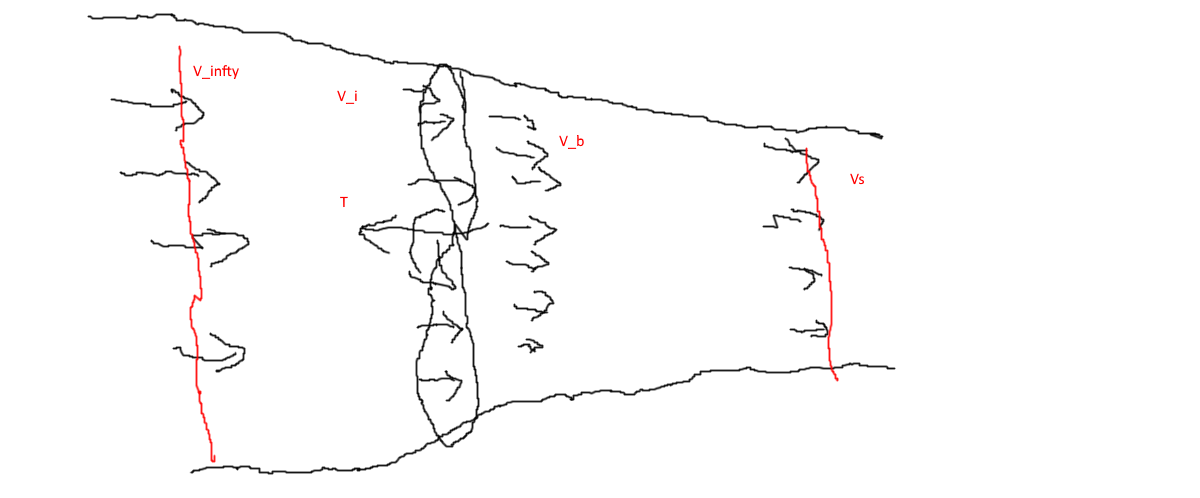
\includegraphics[width=0.7\textwidth]{figs/bem-flow}
\caption{Disc Actuator Propeller Planar Flow}
\label{fig:bem-flow}
\end{figure}
\par
And as such, stemming from classical Disc Actuator$^{\dagger}$ (\emph{momentum}) theory, the force, $T(\Omega)$, acting on the fluid is a function of mass flow rate and change in velocity (pressure differential).
\begin{equation}\label{eq:prop-mass}
\vec{T}=(A_b v_b)\Delta v = \rho \pi R_b^2v_b \Delta v = \rho \pi R_b^2(v_i+v_\infty)\Delta v = \frac{1}{2} \rho \pi R_b^2 \Delta v^2
\end{equation}
Indeed Eq:\ref{eq:prop-mass} can be solved as a function of aerodynamic propulsive power expended, $P=\vec{T}v$. However that relationship between rotational kinetic power transferred is tenuous at best, compounded parasitic losses deteriorate the power transferred. Furthermore, the local fluid velocity over the propeller isn't purely normal to its plane. There are axial and tangential induced velocity components, $a$ and $a'$ respectively. Fluid velocity induction factors can then be defined as a dependents of incident velocity:
\begin{subequations}\label{eq:induction-factors}
\begin{equation}\label{eq:induction-axial}
v_i=a v_\infty
\end{equation}
\vspace{-15pt}
\begin{equation}\label{eq:induction-tangential}
v_\theta=a' \Omega R
\end{equation}
\end{subequations}
From Eq:\ref{eq:induction-factors} the velocity components can be written as functions of free stream velocity $v_\infty$.
\begin{subequations}
\begin{equation}
v_b=(1+a)v_\infty
\end{equation}
\vspace{-15pt}
\begin{equation}
v_s=(1+2a)v_\infty
\end{equation}
\end{subequations}
And from the tangential fluid flow there is then an angular moment rate across the propeller plane too. This produces a torque response to the rotational motion about the propeller's axis of rotation, analogous to Eq:\ref{eq:prop-mass}.
\begin{equation}
\vec{Q}=\rho\pi R_b^3 (v_\theta-v_\infty) v_b 
\end{equation}
Blade-element theory analyses incremental aerofoil sections $dr$ of a propeller profile (Fig:\ref{fig:bem-profile}) at some radius $r$. Net local fluid velocity across a single elemental aerofoil profile $\vec{U}$ is calculated as:
\begin{equation}
\vec{U}=\sqrt{(v_\infty+v_i)^2+(v_\Omega+v_\theta)^2}
\end{equation}
\begin{figure}[htbp]
\centering
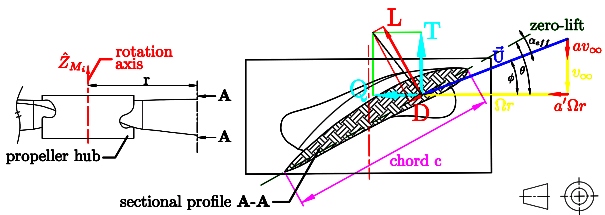
\includegraphics[width=0.9\textwidth]{figs/bem-profile}
\caption{Blade element profile at radius r}
\label{fig:bem-profile}
\end{figure}
Each elemental profile, of chord length $c$, has a local pitch, $\theta$, of its aerofoil profile relative to the horizontal. Local fluid velocities (again in Fig:\ref{fig:bem-profile}) encountered by the propeller make their own an angle of attack $\phi$ such that:
\begin{equation}
\phi=\theta-\alpha_{effective}
\end{equation}
That local angle of attack changes with the inflow magnitude $v_\infty$ and the induced axial velocity $v_i$. That trigonometric ratio is given as:
\begin{equation}
\phi=tan^{-1}\bigg(\frac{v_\infty+v_i}{v_\Omega+v_\theta}\bigg)=tan^{-1}\bigg(\frac{v_\infty(1+a)}{\Omega r(1+a')}\bigg)
\end{equation}
\par
The in-plane fluid flow $\vec{U}(r,\phi)$, for an element at radius $r$ with a local angle of attack $\phi$, then contributes towards elemental lift and drag forces as a function of aerofoil's dimensionless lift, $C_L$, and drag, $C_D$, coefficients\footnote{The lift and drag coefficients are determined by the aerofoil's characteristics, but would be constant across the length of a variable pitch, non-twisted hinged propeller\ldots}.
\begin{subequations}
\begin{equation}
\Delta L=\frac{1}{2}\rho \vec{U}(r,\phi)^2 c C_L
\end{equation}
\vspace{-10pt}
\begin{equation}
\Delta D=\frac{1}{2}\rho \vec{U}(r,\phi)^2 c C_D
\end{equation}
\end{subequations}
With air density $\rho$\footnote{Typically $\rho = 1.225 kg/m^3$} and local chord length $c$. Those lift and drag forces are taken as components parallel and perpendicular to the plane of rotation. Those components are then thrust $T$ and torque $F_x$ forces (Fig:\ref{fig:bem-profile}).
\begin{subequations}
\begin{equation}\label{eq:element-thrust}
dT=\frac{1}{2}\rho\vec{U}(r,\phi)^2c\big(C_L cos(\phi)+C_D sin(\phi)\big).dr
\end{equation}
\vspace{-10pt}
\begin{equation}\label{eq:element-drag}
dF_x=\frac{1}{2}\rho\vec{U}(r,\phi)^2c\big(C_L sin(\phi)+C_D cos(\phi)\big).dr
\end{equation}
\vspace{-10pt}
\begin{equation}\label{eq:element-torque}
\rightarrow dQ = \frac{1}{2}\rho\vec{U}(r,\phi)^2c\big(C_L sin(\phi)+C_D cos(\phi)\big)r.dr
\end{equation}
\vspace{-10pt}
\begin{equation}\label{eq:element-power}
\rightarrow dP = \Omega r dF_x .dr
\end{equation}
\end{subequations}
Typically a power term, Eq:\ref{eq:element-power}, is given in lieu of torque or drag terms, Eq:\ref{eq:element-torque} or Eq:\ref{eq:element-drag}. Then calculating forces and torques as per momentum theory for each element, in terms of tangential and axial induction factors:
\begin{subequations}
\begin{equation}
dT=\rho 4 \pi r^2 v_\infty(1+a)a.dr
\end{equation}
\vspace{-10pt}
\begin{equation}
dP=\rho 4 \pi r^2 v_\infty(1+a)\Omega r (1+a').dr
\end{equation}
\end{subequations}
Then equating momentum and element terms together produces the blade-element momentum equation(s) for thrust and power produced by a propeller. Following a few assumptions, most importantly that the lift coefficient $C_L$ is a linear function of the effective angle of attack $\alpha_{eff}$. The lift curve gradient ,$a_L$, for an ideally twisted blade, like the fixed pitch propellers under consideration here, is typically $2\pi$ such that $C_L=2\pi(\theta-\phi)$. And assuming that tangential induced velocities $v_\theta$ are small (or that the tangential induction factor $a'<<1$) when compared to the propeller's speed $\Omega r$. Similarly the net inflow and axial induced velocities $v_\infty + v_i<<\Omega r$.\footnote{Small angle approximations then apply to $cos(\phi+\alpha_{eff})\approx 1$ and $sin(\phi+\alpha_{eff})\approx \phi+\alpha_{eff}$}
\begin{subequations}
\begin{equation}\label{eq:bem-thrust}
T=\int_{r=0}^R \frac{1}{2} a_L b c \rho (\Omega r)^2 \big(\theta-\frac{v_\infty+v_i}{\Omega r}\big).dr
\end{equation}
\vspace{-5pt}
\begin{equation}\label{eq:bem-power}
P=\int_{r=0}^R \frac{1}{2}a_L b c \rho (\Omega r)^3\bigg[\big(\theta-\frac{v_\infty+v_i}{\Omega r}\big)\big(\frac{v_\infty+v_i}{\Omega r}\big) + C_d\bigg].dr
\end{equation}
\end{subequations}
Generally knowing the exact pitch and chord values as a function $r/R$ is difficult and calculating integrals at each process step is cumbersome. Both Eq:\ref{eq:bem-thrust} \& Eq:\ref{eq:bem-power} can be solved by equating element and momentum terms (Appendix:\ref{}). Often dimensionless thrust, torque and power coefficients are defined:
\begin{subequations}\label{eq:coefficients}
\begin{equation}\label{eq:thrust-coefficient}
C_T(J)=\frac{T}{\rho \Omega^2 D^4}
\end{equation}
\vspace{-10pt}
\begin{equation}\label{eq:power-coefficient}
C_P(J)=\frac{P}{\rho \Omega^3 D^5}
\end{equation}
\end{subequations}
\begin{minipage}{\textwidth}
\begin{wrapfigure}{r}{0.5\textwidth}
\vspace{-17pt}
\centering
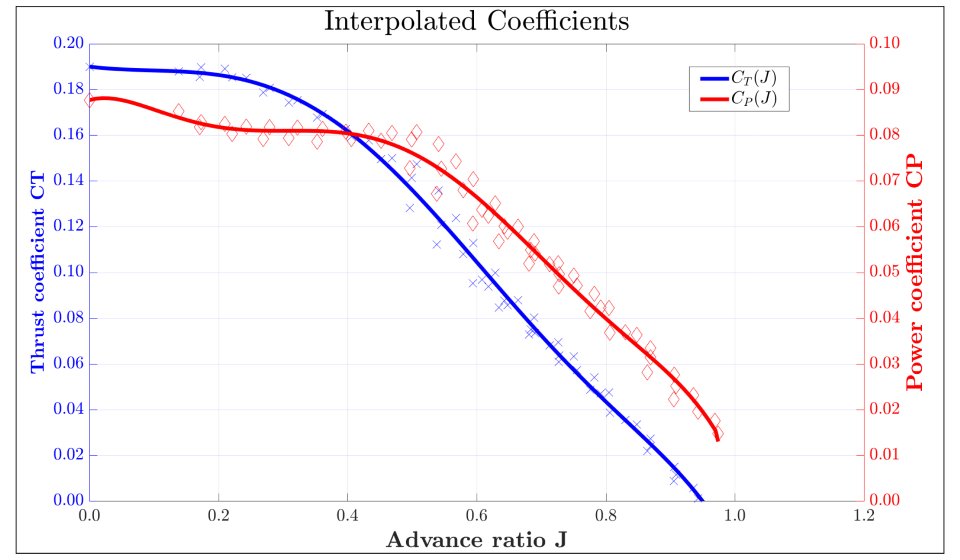
\includegraphics[width=0.5\textwidth]{graphs/coeffs-plot}
\vspace{-15pt}
\caption{Power \& thrust coefficients}
\label{fig:coeffs-plot}
\end{wrapfigure}
Where $\Omega$ is the propellers rotational speed in RPS and $D$ is the propellers diameter. For fixed pitch propellers the thrust and power coefficients are easily determined. Eq:\ref{eq:thrust-coefficient} and Eq:\ref{eq:power-coefficient} both vary due to the \emph{advance ratio} $J$.
\begin{equation}\label{eq:advance}
J = \frac{v_\infty}{\Omega R}
\end{equation}
In most cases, the net head stream velocity $v_\infty$ is the perpendicular component (projected onto the plane's normal vector $\hat{n}$) of the vehicles transnational velocity in the body frame, $\vec{v}_b\cdot\hat{n}$. For the case of a zero advance ratio, $J=0$, the conditions are regarded as static. Static thrust and power coefficients are nominal in their values. 
\end{minipage}
\par
\vspace{20pt}
\par
Propeller databases like \cite{UIUC}\footnote{The UIUC database also includes blade profiles, pitch and chord lengths. The database is the outcome of \cite{lowreynolds}.} provide comprehensive values for a range of propeller types at different advance ratios. The introduction of those coefficients greatly simplifies the thrust estimation process. For a typical 6X4.5 inch propeller\footnote{linearly interpolated from similar pitched database results to match physical test values}, the static thrust and power coefficients respectively are:
\begin{subequations}
\begin{equation}
{\color{blue}C_{T0}}=0.191
\end{equation}
\vspace{-20pt}
\begin{equation}
{\color{red}C_{P0}}=0.0877
\end{equation}
\end{subequations}
Fig:\ref{fig:coeffs-plot} shows the thrust, {\color{Blue}$C_{T}$}, and power, {\color{Red}$C_{P}$}, coefficients as a function of the advance ratio J. As the incident head fluid velocity, $v_\infty$, increases, the thrust coefficient decreases. So too does the power coefficient and hence the aerodynamic torque. 
\begin{figure}[htbp]
\begin{subfigure}{0.5\textwidth}
\centering
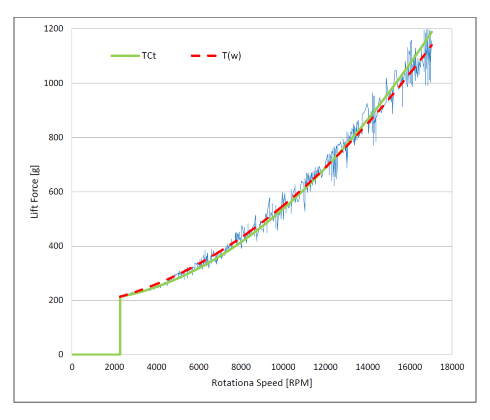
\includegraphics[width=\textwidth]{graphs/thrust-plot}
\caption{Thrust plot}
\label{fig:thrust-plot}
\end{subfigure}
\begin{subfigure}{0.5\textwidth}
\centering
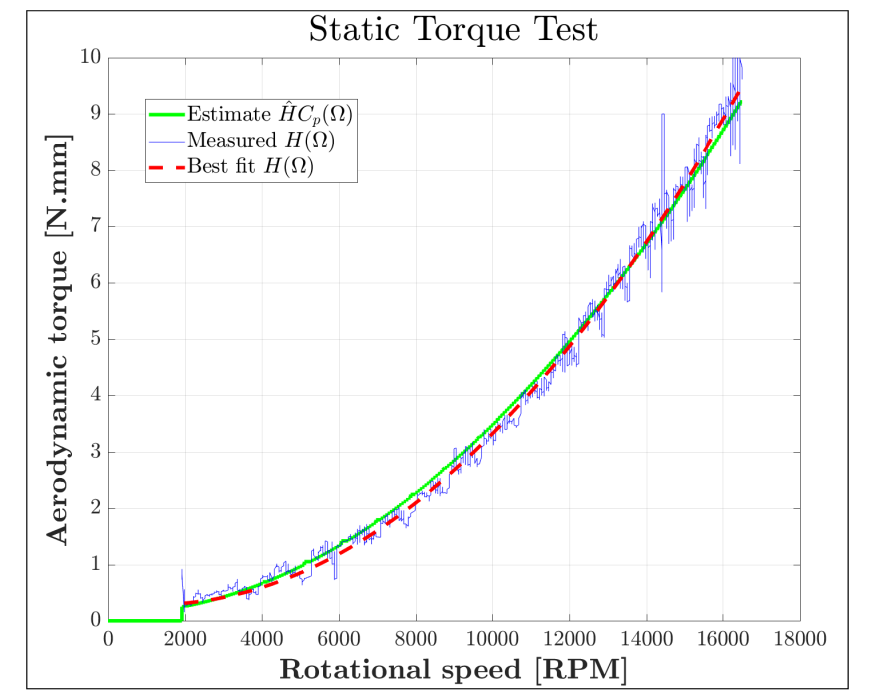
\includegraphics[width=\textwidth]{graphs/torque-plot}
\caption{Torque plot}
\label{fig:torque-plot}
\end{subfigure}
\caption{Static propeller tests}
\label{fig:propeller-plots}
\end{figure}
\par
In Fig:\ref{fig:propeller-plots}, the results both of static thrust and torque tests are plotted. In each test the measured values are shown (with quadratic trend-lines) and an estimated value dependent on static coefficients. Using the results from the plot in Fig:\ref{fig:coeffs-plot} as a lookup table and calculating the values from Eq:\ref{eq:coefficients}, induced propeller thrust and torques can be accurately modeled (\emph{quadratically}\footnote{The power term is cubic W.R.T its coefficient}). Instantaneous advance ratios, or rather the propeller incident fluid flow(s), are dependent on the vehicle's net transnational and angular velocity. Such that the fluid velocity's normal component to the propeller plane is given by:
\begin{equation}
v_\infty = (\vec{v}_b + \vec{L}_{arm}\times \vec{\omega}_b)\cdot \hat{n}
\end{equation}
Where $\vec{v}_b$ is the body's transnational velocity and $\vec{\omega}_b$ is the body's angular velocity, both transformed to the propeller's frame, $\in\mathcal{F}^{M_i}$. Additionally $\hat{n}$ is a unit vector normal to the propeller's rotational plane. Then $J$ is calculated as in Eq:\ref{eq:advance}.
\par
{\color{Gray}\emph{It's worth noting that the above static coefficients are indeed calculated from physical static tests. However advance ratio coefficient dependencies are linearly interpolated from the closest available matching data (APC Thin-Electric 8X6 propellers). Discrepancies between the model or coefficient values derived can be accounted for with lumped uncertainty and disturbance term(s). Model uncertainty compensation is elegantly incorporated in adaptive backstepping or $H_\infty$ control algorithms. The deviation of the modeled thrust or torques from their true values would be easy to incorporate into a plant dependent Lyupanov candidate function; Section:\ref{.}.}}
%====================================================
\subsection{Hinged Propeller Conning \& Flapping}
\label{subsec:dynamics.aero.flap}
%====================================================
Other common non-linear aerodynamic effects which deteriorate a propellers performance are that of conning and flapping. Both effects are significantly more pronounced in the context of hinged, variable pitch propellers. The prototype under consideration here has fixed pitch, rigid propellers and as such neither conning nor propeller flapping are significant to adversely act on the system. With that being said, they are worth mentioning briefly.
\par

%====================================================
\subsection{Vortex Ring State}
\label{subsec:dynamics.aero.vrs}
%====================================================
\subsection{Drag}
\label{subsec:dynamics.aero.drag}
%====================================================

%====================================================
\section{Consolidated Model}
\label{sec:dynamics.model}%====================================================
Consolidating